\subsection{Giao diện chia sẻ workspace}

\begin{figure}[H]
    \centering
    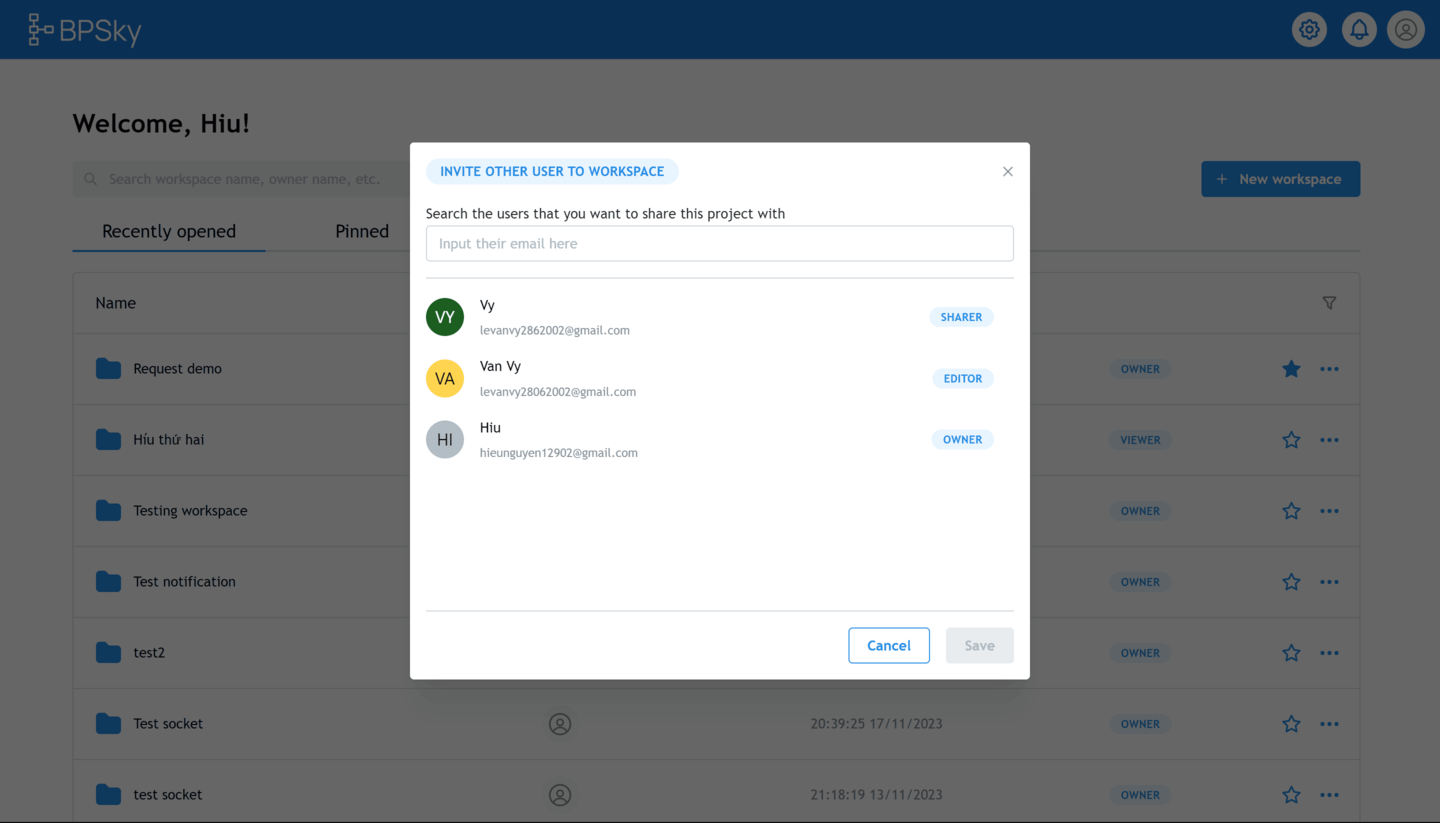
\includegraphics[ width = 0.7\linewidth]{Content/Hiện thực hệ thống/documents/Hiện thực giao diện người dùng/images/ShareModal.png}
    \vspace{0.5cm}
    \caption{Giao diện share modal khi người dùng muốn mời/gửi yêu cầu mời người dùng khác vào workspace}
    \label{fig: Giao diện share modal khi người dùng muốn mời/gửi yêu cầu mời người dùng khác vào workspace}
\end{figure}

Người dùng có thể mời người dùng khác vào workspace bằng cách chọn "Share" từ dropdown menu. Sau khi chọn, hệ thống sẽ hiển thị giao diện share modal như hình \ref{fig: Giao diện share modal khi người dùng muốn mời/gửi yêu cầu mời người dùng khác vào workspace}. Tại đây, người dùng có thể nhập tên người dùng mà mình muốn mời vào workspace, sau đó chọn quyền hạn của người được mời vào - quyền hạn của người này không được phép cao hơn người gửi lời mời (owner > editor > sharer > viewer). Sau khi hoàn tất, người dùng có thể chọn "Share" để mời người dùng vào workspace hoặc "Cancel" để hủy thao tác.